\documentclass[11pt]{article}
\usepackage[margin=1in]{geometry}
\usepackage{amsmath,amssymb}
\usepackage{booktabs}
\usepackage{hyperref}
\usepackage{listings}
\usepackage{xcolor}
\usepackage{graphicx}
\usepackage{caption}

\lstset{
  language=Python,
  basicstyle=\ttfamily\small,
  keywordstyle=\color{blue!70!black},
  commentstyle=\color{gray},
  breaklines=true,
  frame=single,
  xleftmargin=1em,
  columns=fullflexible,
}

\hypersetup{colorlinks,linkcolor=blue!60!black,citecolor=blue!60!black,urlcolor=blue!60!black}

\title{Notes on ``Neural Thickets''}
\author{
Codex 5.4\thanks{Experiments and analysis code.} \quad
Claude Opus 4.6\thanks{Writeup.} \quad
Andy Arditi\thanks{Supervision and direction.}
}
\date{March 2026}

\begin{document}
\maketitle

\section{The Paper's Core Claims}\label{sec:paper}

Gan \& Isola~\cite{gan2026thickets} study the local neighborhood of pretrained LLM weights. They define \emph{solution density} as the probability that a random Gaussian perturbation improves task performance:
\begin{equation}\label{eq:density}
  \delta(m) \;=\; \Pr_{\boldsymbol{\epsilon}\sim\mathcal{N}(\mathbf{0},\,\sigma^2\mathbf{I})}\!\bigl[\,s(\boldsymbol{\theta}+\boldsymbol{\epsilon}) \;\ge\; s(\boldsymbol{\theta})+m\,\bigr]
\end{equation}
where $\boldsymbol{\theta}\in\mathbb{R}^d$ are the pretrained weights, $s$ is a task metric, and $\sigma$ controls the perturbation radius. The perturbation model is $\boldsymbol{\theta}' = \boldsymbol{\theta} + \sigma\cdot\boldsymbol{\epsilon}(s)$ with $\boldsymbol{\epsilon}$ drawn from an isotropic Gaussian over the full parameter space.

The paper makes three core claims:

\begin{enumerate}
  \item \textbf{Density scales with model size.} $\delta(m)$ increases monotonically from 0.5B to 32B parameters.
  \item \textbf{Perturbations are diverse specialists.} A measure called Spectral Discordance $\mathcal{D}$ increases with scale, indicating that different perturbations improve different tasks.
  \item \textbf{RandOpt is competitive.} A simple algorithm---sample $N$ perturbations, evaluate on a training set, ensemble the top $K$ via majority vote---matches PPO, GRPO, and ES on several benchmarks.
\end{enumerate}

\subsection{How the paper measures these claims}\label{sec:paper_method}

\paragraph{Density (Claim 1).} The paper samples 1000 random Gaussian perturbations with $\sigma=0.005$ for each model in the Qwen-2.5 family (0.5B, 1.5B, 3B, 7B, 32B instruction-tuned variants). Each perturbed model is evaluated on three reasoning tasks (GSM8K, OlympiadBench, Countdown). The density $\delta(m)$ is computed as the fraction of perturbations whose task accuracy exceeds the base model's accuracy by at least $m$. This is reported in their Figure~3 for several thresholds $m$. The same $\sigma=0.005$ is used for all model sizes.

\paragraph{Diversity (Claim 2).} 500 perturbations are evaluated across seven tasks. For each perturbation, the percentile rank (relative to the population) is computed per task, yielding a matrix $\mathbf{P}\in[0,1]^{500\times 7}$. The Spectral Discordance $\mathcal{D}=1-\frac{1}{M(M-1)}\sum_{j\neq k}\mathbf{C}_{jk}$ is computed from the inter-task correlation matrix $\mathbf{C}$ of this matrix. High $\mathcal{D}$ means perturbations that help one task tend to hurt others (specialists); low $\mathcal{D}$ means perturbations help or hurt all tasks together (generalists).

\paragraph{RandOpt (Claim 3).} $N=5000$ perturbations are sampled, each assigned a $\sigma$ drawn uniformly from a set $\Sigma$ (typically $\{0.001, 0.002, 0.003\}$). Each perturbed model is evaluated on a training split of 200 samples. The top $K=50$ by training accuracy are selected. At test time, all $K$ models generate answers for each test input and the final prediction is the majority vote.

\paragraph{} All three measurements assume that the perturbation $\boldsymbol{\epsilon}$ is drawn from an isotropic Gaussian over the full parameter space. The density definition (Eq.~\ref{eq:density}) and the theoretical discussion (their Sections 1--2) are stated in terms of this distribution explicitly.

\subsection{Scope of this note}\label{sec:scope}

We focus on \textbf{Countdown}, the paper's primary evaluation task. We test Claims~1 and~3 (density and RandOpt) on the Qwen-2.5-Instruct family at 0.5B, 1.5B, 3B, and 7B. Since measuring density requires sampling $N$ perturbations and evaluating each on the training set, the additional cost of also running the RandOpt ensemble (evaluating the top $K$ on the test set) is marginal, so we report both.

We do \emph{not} test Claim~2 (diversity / Spectral Discordance), which requires multi-task evaluation. We also do not compare against the PPO, GRPO, or ES baselines, and we do not test models beyond the Qwen-2.5 family or scales beyond 7B.


\section{Issue 1: The Perturbation Sampler Does Not Match the Math}\label{sec:rng}

\subsection{The bug}

The paper's perturbation model requires drawing $\boldsymbol{\epsilon}\sim\mathcal{N}(\mathbf{0},\mathbf{I}_d)$---a single independent noise vector across all $d$ parameters. The released implementation does something different. In \texttt{utils/worker\_extn.py}\footnote{\url{https://github.com/sunrainyg/RandOpt/blob/60061828e3d378d74faa09cb14c2410db820391d/utils/worker_extn.py\#L69-L83}.}, the perturbation loop is:

\begin{lstlisting}
def perturb_self_weights(self, seed, noise_scale, negate=False):
    self._set_seed(seed)
    scale = float(noise_scale)
    sign = -1.0 if negate else 1.0
    for name, p in self.model_runner.model.named_parameters():
        gen = torch.Generator(device=p.device)
        gen.manual_seed(int(seed))  # same seed every iteration
        noise = torch.randn(p.shape, ..., generator=gen)
        if self._should_perturb(name):
            p.data.add_(sign * scale * noise)
\end{lstlisting}

A fresh \texttt{Generator} is created and seeded to the \emph{same value} for every parameter tensor. This means every same-shaped tensor receives byte-for-byte identical noise. In a Qwen-2.5 transformer, \texttt{q\_proj} and \texttt{o\_proj} across all layers share a shape and therefore receive identical perturbations; similarly for \texttt{k\_proj}/\texttt{v\_proj}, \texttt{gate\_proj}/\texttt{up\_proj}, etc.

\paragraph{Impact on effective dimensionality.} For Qwen-2.5-3B ($\sim$324 parameter tensors), there are only $\sim$5 unique shapes, with up to 72 tensors per shape group. The effective perturbation dimensionality is $\sim$28M, not the $\sim$1.6B that isotropic Gaussian noise would use---a $\sim$57$\times$ reduction. The perturbation is closer to a single ``layer-edit template'' stamped identically across the network than to random noise in billion-dimensional space.

\paragraph{What the correct implementation looks like.} The fix is to create one generator per device, seed it once before the loop, and let it advance naturally. This is what the paper's separate reproduction utility (\texttt{utils/repro\_seed.py}) already does---and what the toy 1D experiments (\texttt{1D\_signals\_expts/models.py}) also do. Only the main LLM code path has the bug, meaning the reproduction utility would produce different models than those actually evaluated.

\subsection{Empirical test}\label{sec:rng_expt}

We modified the codebase to support both perturbation modes via a command-line flag: \texttt{per\_parameter} (released behavior, correlated noise) and \texttt{global\_stream} (one generator advancing across all tensors, true isotropic Gaussian). We ran RandOpt on Countdown with both samplers across all four model sizes. Each run uses the same dataset split, global seed, mixed-sigma population ($\sigma\in\{0.0005, 0.001, 0.002, 0.003, 0.005\}$), and selection protocol ($N=40$, 100 train / 100 test). The only variable is the perturbation mode.

\subsection{Results}

\begin{figure}[t]
\centering
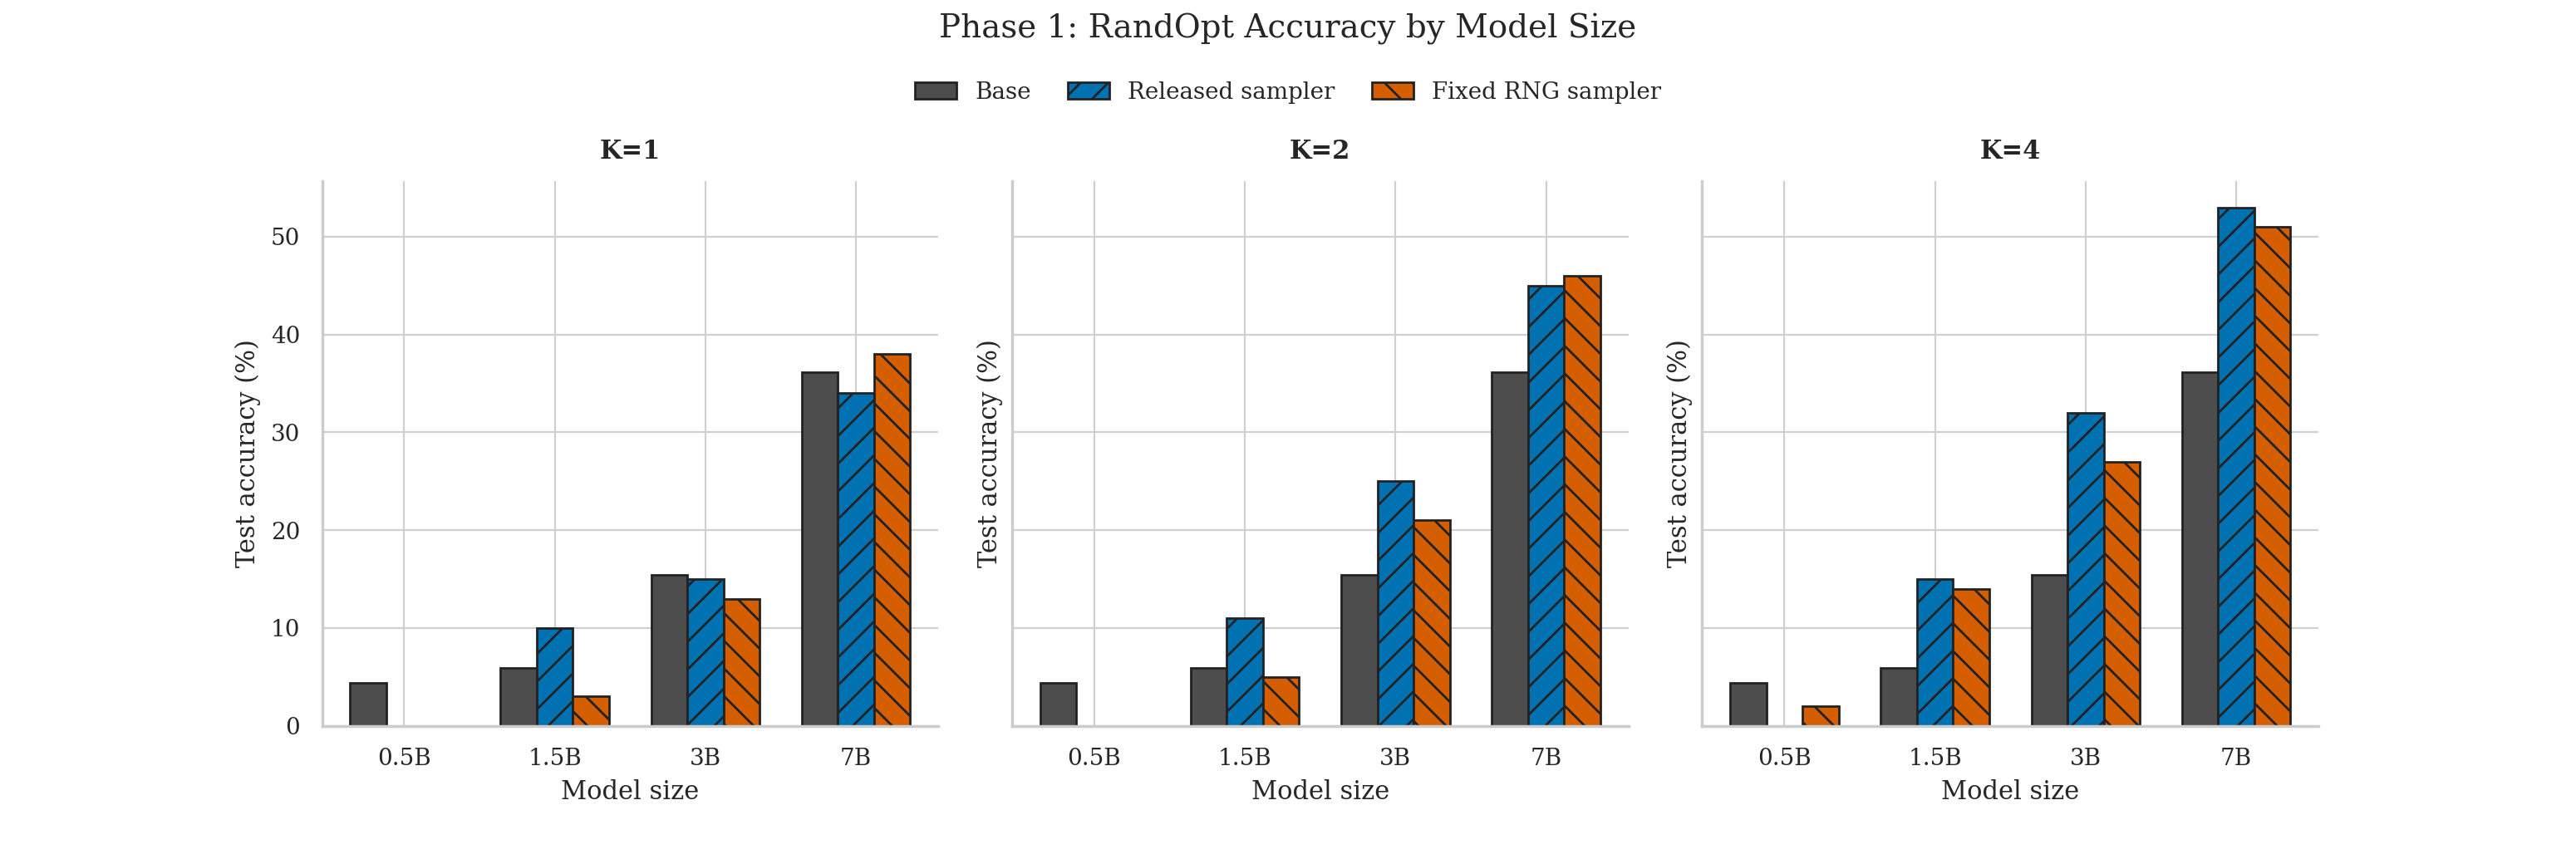
\includegraphics[width=\textwidth]{figures/phase1_accuracy.png}
\caption{RandOpt ensemble accuracy on Countdown under the released (correlated) and corrected (isotropic) samplers. $N=40$, mixed $\sigma$, 100 train / 100 test samples. The released sampler is modestly better at 1.5B and 3B, especially at small $K$. At 7B, the corrected sampler is comparable. At no scale does fixing the RNG cause the method to collapse.}\label{fig:rng_ab}
\end{figure}

Figure~\ref{fig:rng_ab} shows the A/B comparison. The released (correlated) sampler outperforms the corrected sampler at 1.5B and 3B, particularly at $K=1$ and $K=2$, while at 7B the two samplers are comparable or the corrected sampler is slightly better. At 0.5B, neither sampler produces useful results at these small $N$ and $K$ values (though the paper reports 8.4\% on Countdown with $N=5000$, $K=50$ using the released sampler).

\paragraph{Caveats.} This comparison uses $N=40$ with a 100-sample train/test split, so the numbers are noisy---individual accuracy values could shift by $\sim$5--10 percentage points with different random seeds. The qualitative pattern (corrected sampler doesn't collapse, released sampler has a modest edge at smaller scales) is more reliable than the specific numbers.

\paragraph{Discussion.} The fact that the 57$\times$ dimensionality reduction from the RNG bug produces only a modest performance difference is itself surprising. One possible explanation is that the most functionally important parameters---embedding and unembedding matrices---have unique shapes and therefore receive distinct noise under either sampler. We have not tested this hypothesis directly. Another possibility is that the thicket phenomenon is inherently low-dimensional, so the reduced search space of the correlated sampler is not much of a handicap. Regardless, the bug means the paper's experiments do not test the distribution described in their math, even if the practical conclusions are similar.


\section{Issue 2: Fixed $\sigma$ Across Model Scales}\label{sec:sigma}

The paper uses $\sigma=0.005$ for all density measurements from 0.5B to 32B. But the same per-parameter noise magnitude has vastly different functional impact at different scales. There is a simple theoretical reason for this: for a single linear layer $y = Wx$ with fan-in $n$, a per-parameter perturbation of magnitude $\sigma$ produces an output perturbation of magnitude $\sigma\sqrt{n}$ (see Appendix~\ref{app:norms}). Wider matrices amplify noise. Since larger models are wider, the same $\sigma$ is functionally more disruptive for larger models.

The paper's own Figure~12 shows the empirical consequence: at $\sigma=0.005$, the fraction of perturbations that improve GSM8K accuracy is 0\% at 0.5B, 18\% at 1.5B, 37\% at 3B, and 64\% at 32B. The density scaling law (Claim~1) is therefore confounded: it could reflect genuine geometric structure \emph{or} simply that $\sigma=0.005$ is catastrophically large for small models and nearly negligible for large ones.

\subsection{Log-spaced sigma sweep}\label{sec:sigma_expt}

To disentangle sigma sensitivity from the density claim, we ran a log-spaced sigma sweep under the corrected sampler (\texttt{global\_stream}). For each of the four model sizes, we sampled $N=100$ perturbations at each of seven sigma values spanning three orders of magnitude: $\sigma\in\{10^{-5}, 3{\times}10^{-5}, 10^{-4}, 3{\times}10^{-4}, 10^{-3}, 3{\times}10^{-3}, 10^{-2}\}$. We used the paper's data split (200 train / 2000 test samples from Countdown) and measured hit-rate above base training accuracy and $K=1$ test accuracy.

\subsection{Results}

\begin{figure}[t]
\centering
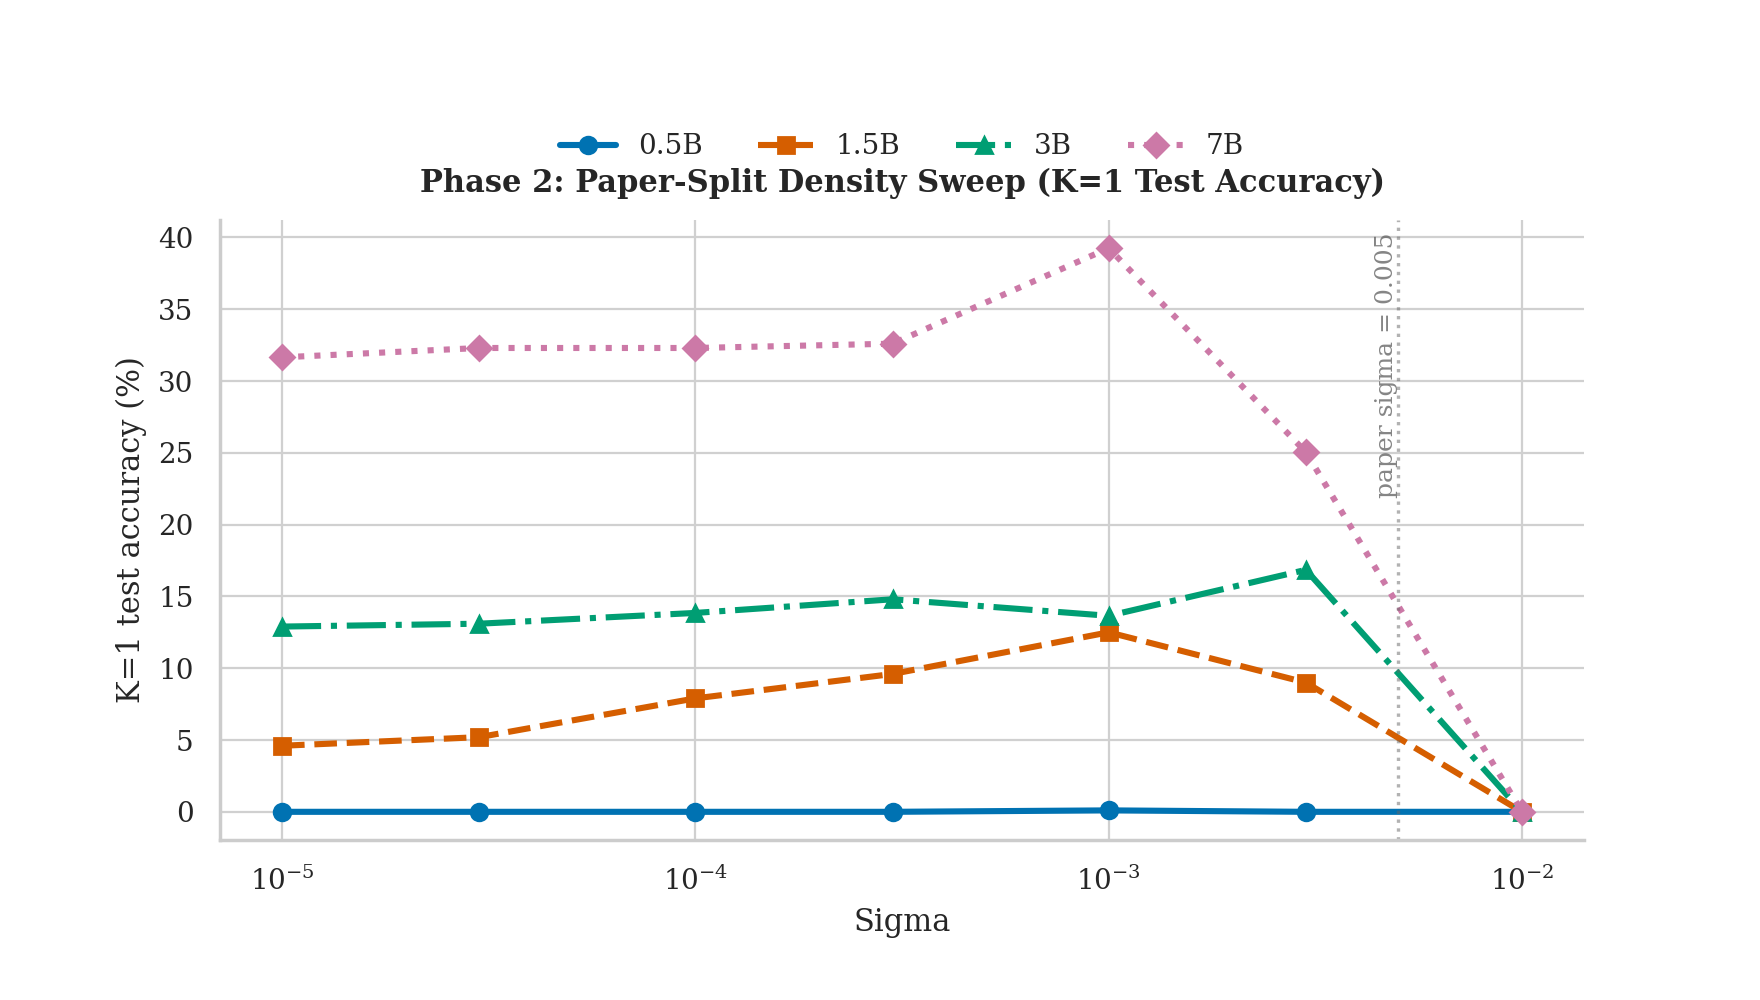
\includegraphics[width=0.85\textwidth]{figures/density_k1_vs_sigma.png}
\caption{$K=1$ test accuracy vs.\ $\sigma$ under the corrected sampler, on the paper's data split (200 train / 2000 test). Each model gets $N=100$ perturbations per $\sigma$. The dashed line marks the paper's $\sigma=0.005$. Our grid brackets this value with $\sigma=0.003$ and $\sigma=0.01$; interpolating, all models appear to be at or near the destructive regime at $\sigma=0.005$. When each model is allowed its own optimal $\sigma$ ($\sim$0.001), peak $K=1$ accuracy scales monotonically with model size.}\label{fig:k1_vs_sigma}
\end{figure}

Figure~\ref{fig:k1_vs_sigma} is the central result. Several observations:

\begin{enumerate}
\item \textbf{The paper's $\sigma=0.005$ appears to be in the destructive range.} Our grid does not include $\sigma=0.005$ exactly, but the surrounding points ($\sigma=0.003$ and $\sigma=0.01$) show near-zero accuracy for all models, placing the paper's value at or beyond the productive regime. The productive range under the corrected sampler is roughly $\sigma\in[10^{-4}, 3{\times}10^{-3}]$.

\item \textbf{Peak $K=1$ accuracy scales monotonically with model size.} When each model is evaluated at its best $\sigma$: 0.1\% (0.5B) $<$ 12.5\% (1.5B) $<$ 16.9\% (3B) $<$ 39.3\% (7B). This is consistent with the paper's qualitative claim that larger models have richer neighborhoods---but only once $\sigma$ is chosen appropriately per model. Note that $K=1$ accuracy is not the same quantity as the paper's density $\delta(m)$; the hit-rate plots (Figure~\ref{fig:hitrate_vs_sigma}) tell a more nuanced story, with monotonic scaling holding at $m=0$ but not cleanly at stricter margins.

\item \textbf{7B is robust across a wide range of $\sigma$.} Its accuracy is $\sim$32\% even at $\sigma=10^{-5}$, because 7B's base accuracy is already $\sim$32\% on Countdown---the perturbation barely moves the model at very small $\sigma$. It peaks at $\sim$39\% near $\sigma=10^{-3}$.

\item \textbf{0.5B shows minimal improvement at any $\sigma$.} $K=1$ accuracy is near 0\% across the full sweep. However, the hit-rate data (Figure~\ref{fig:hitrate_vs_sigma}) shows that perturbations \emph{do} improve the 0.5B model on the training set at small $\sigma$---the improvements are just too small to produce useful $K=1$ test accuracy with $N=100$. The paper reports 8.4\% on Countdown with 0.5B using $N=5000$ and $K=50$, demonstrating that much larger population and ensemble sizes can extract something even at this scale. Our $N=100$, $K=1$ setup is too underpowered to see this.

\item \textbf{Optimal $\sigma$ is similar across the productive scales.} All three models that show clear improvement (1.5B, 3B, 7B) peak near $\sigma\approx 0.001$. The toy model in Appendix~\ref{app:norms} predicts a $\sim$1.5$\times$ difference between 1.5B and 7B ($\sigma_{\text{opt}}\propto 1/(\sqrt{\text{width}}\cdot L)$), which is within the resolution of our log-spaced grid. A finer grid would be needed to test this prediction.
\end{enumerate}

\begin{figure}[t]
\centering
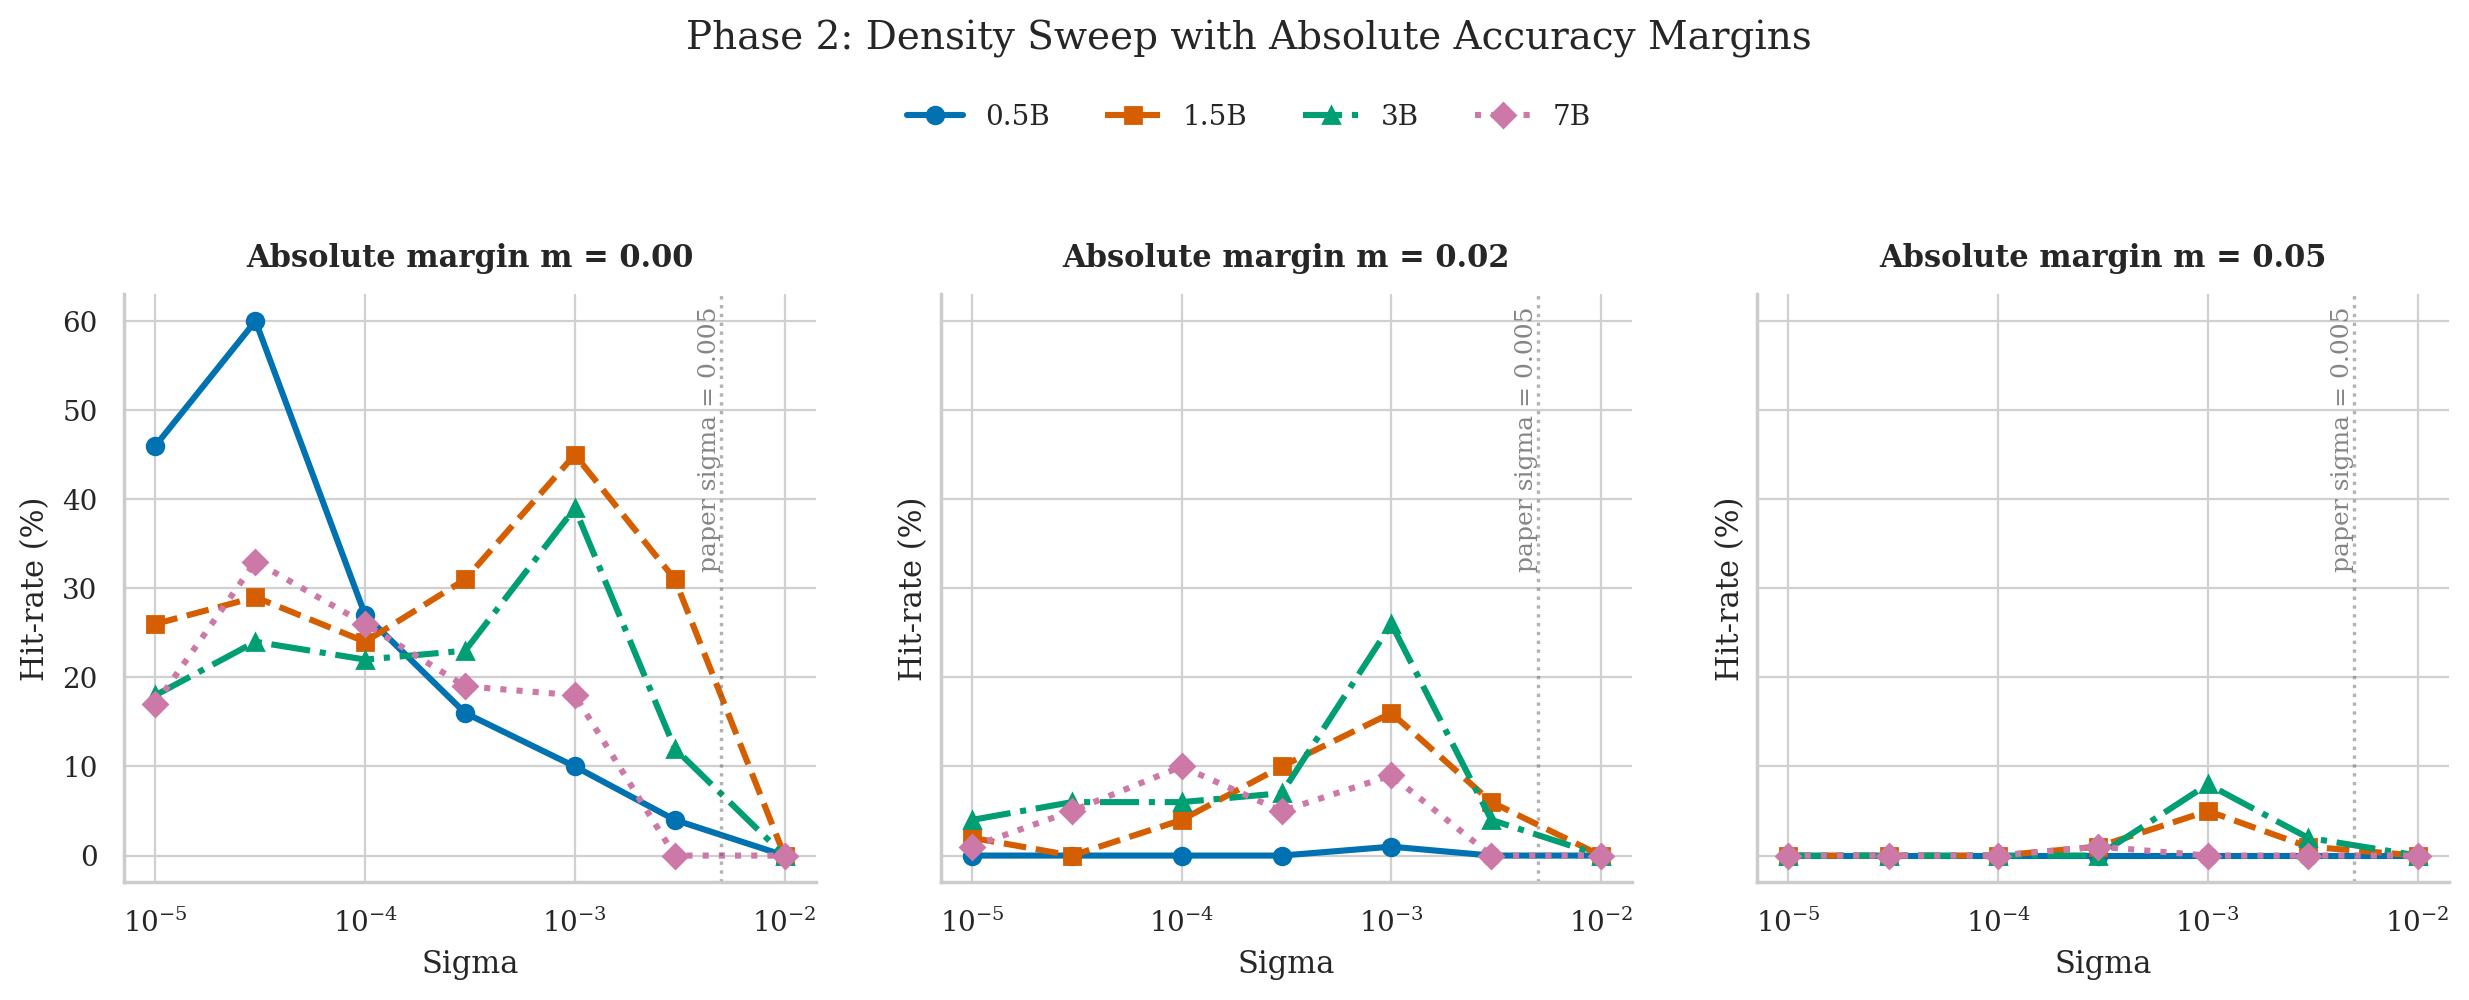
\includegraphics[width=\textwidth]{figures/density_hitrate_vs_sigma.png}
\caption{Hit-rate (fraction of perturbations exceeding base accuracy by at least margin $m$) vs.\ $\sigma$, under the corrected sampler. Left: $m=0$ (any improvement). Center: $m=0.02$. Right: $m=0.05$. At $m=0$, all models show nonzero hit-rates; at stricter margins, larger models generally retain higher hit-rates, though the ordering is not cleanly monotonic at all $\sigma$ values. The curves are noisy at $N=100$.}\label{fig:hitrate_vs_sigma}
\end{figure}

Figure~\ref{fig:hitrate_vs_sigma} shows hit-rate curves at different accuracy margins. At $m=0$ (any improvement over base), all models---including 0.5B---show nonzero hit-rates in the $\sigma\in[10^{-4}, 10^{-3}]$ range. At higher margins ($m=0.02$, $m=0.05$), only the larger models retain meaningful hit-rates.


\section{Issue 3: Parameter Scales Are Not Uniform}\label{sec:scales}

Even within a single model, a fixed $\sigma$ does not treat all parameters equally in any meaningful sense. We computed per-tensor weight statistics across the Qwen-2.5 family (Figures~\ref{fig:weight_scales}--\ref{fig:weight_layers}).

\begin{figure}[t]
\centering
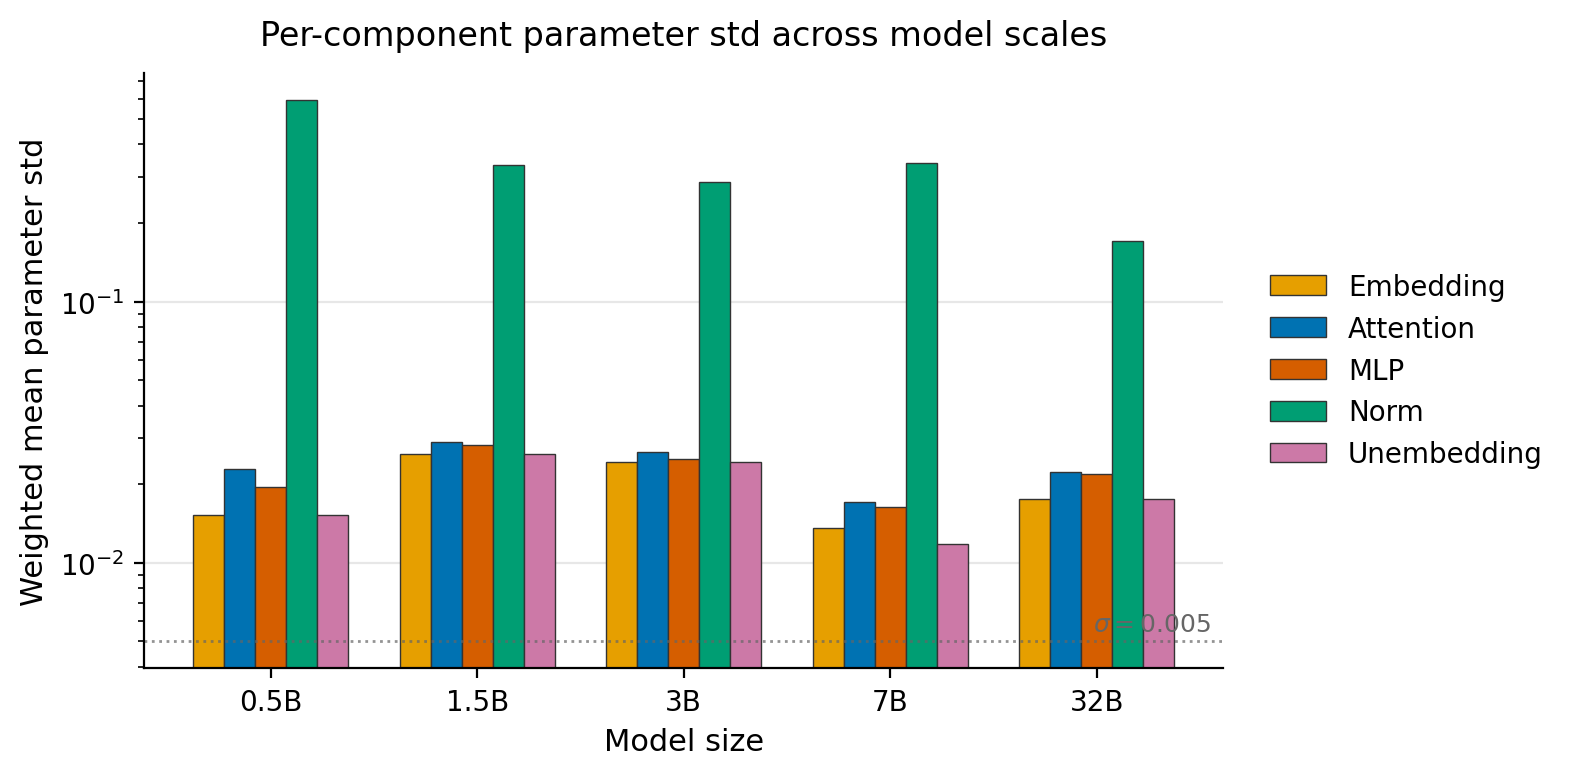
\includegraphics[width=0.75\textwidth]{figures/weight_scale_components.png}
\caption{Weighted mean parameter std by component type across model scales. Embedding, attention, MLP, and unembedding weights all cluster in the $\sim$0.01--0.03 range; norm layers are 10--30$\times$ larger. The dotted line marks $\sigma=0.005$: under the paper's perturbation scheme, weight matrices receive a 20--30\% relative perturbation while norms receive $<$1\%. For 0.5B--3B (tied embeddings), unembedding std equals embedding std; 7B and 32B have separate unembedding matrices. Note that 7B has the smallest weight matrix stds, meaning the same $\sigma$ is relatively more disruptive there.}\label{fig:weight_scales}
\end{figure}

\begin{figure}[t]
\centering
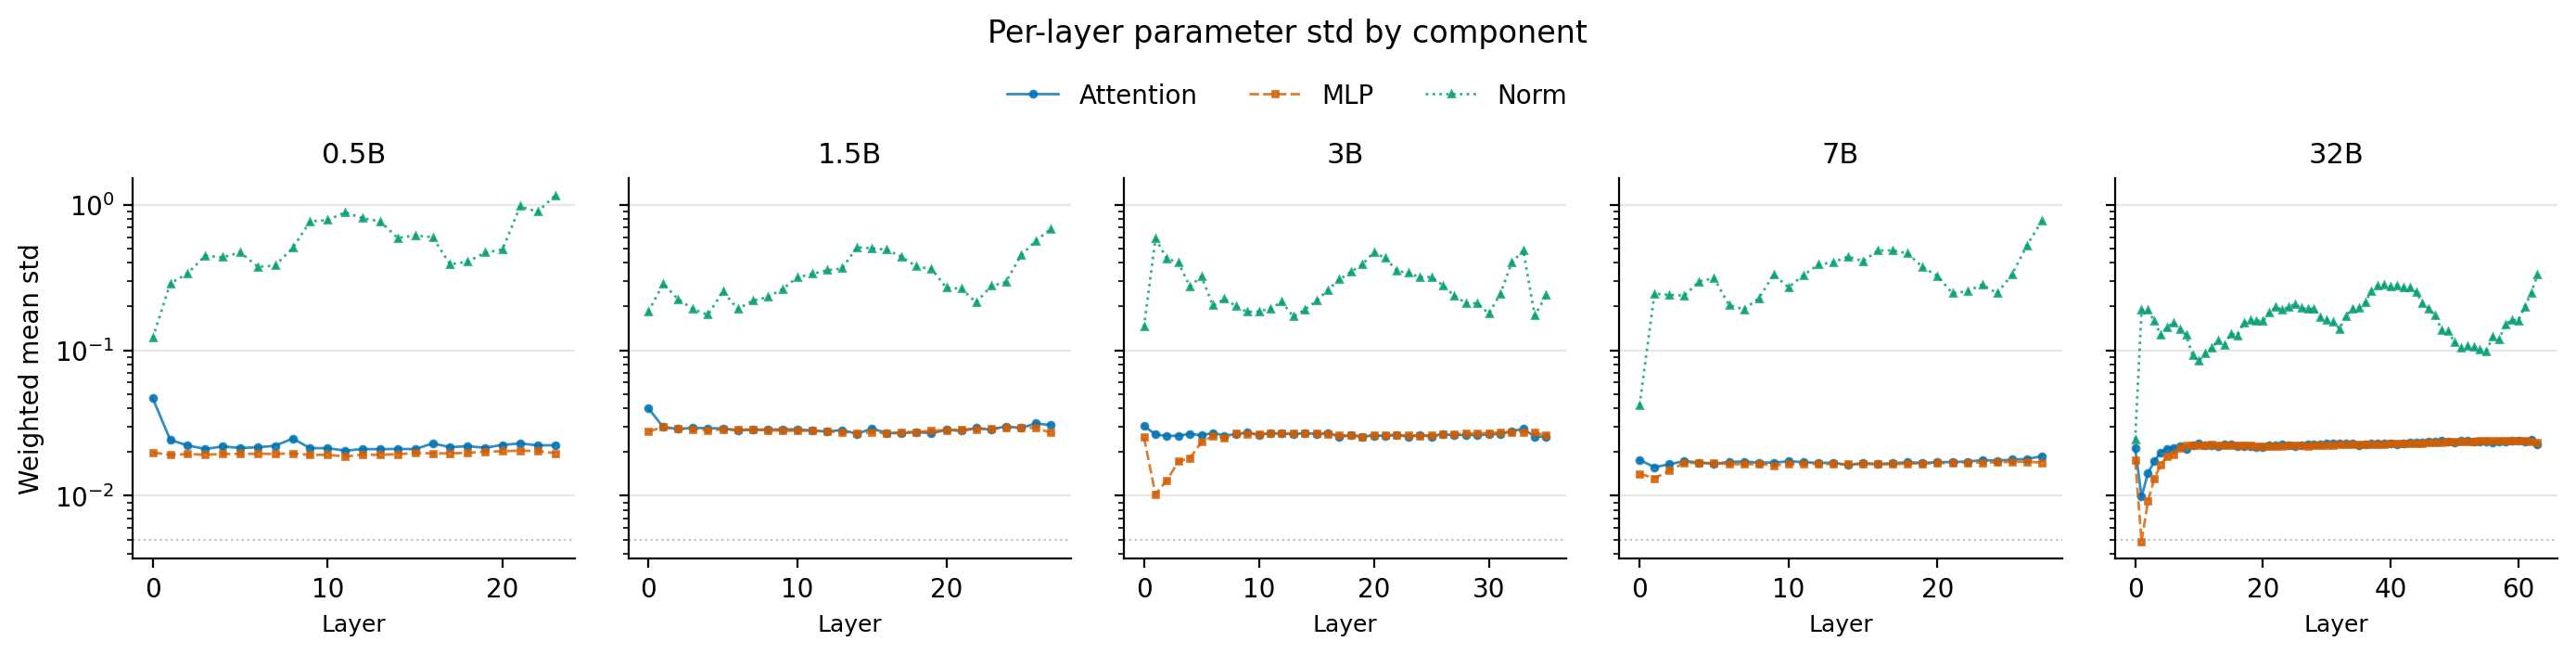
\includegraphics[width=\textwidth]{figures/weight_scale_layers.png}
\caption{Per-layer parameter std by component type across the Qwen-2.5 family. Attention and MLP weights are nearly flat across layers (std $\sim$0.01--0.03), while norm layers vary by over an order of magnitude and show pronounced structure---particularly in early and late layers. The dotted line marks $\sigma=0.005$. At every layer and every scale, norm stds sit 1--2 orders of magnitude above weight matrix stds, reinforcing the observation that a fixed absolute $\sigma$ perturbs these component families very differently.}\label{fig:weight_layers}
\end{figure}

Two observations:

\begin{enumerate}
  \item \textbf{Weight matrix stds are not monotonic in model size.} The 7B model has the smallest per-parameter std (0.016). A fixed $\sigma=0.005$ represents a $\sim$31\% relative perturbation at 7B but only $\sim$18\% at 1.5B. This is consistent with the theoretical expectation from Appendix~\ref{app:norms} that the functional impact of a fixed $\sigma$ grows with width.
  \item \textbf{Norm tensors are 10--30$\times$ larger in std than weight matrices.} Under absolute noise ($\sigma=0.005$), norms receive $\sim$1.5\% relative perturbation while weight matrices receive $\sim$20--30\%. The paper's scheme effectively searches over weight matrix edits while leaving norms nearly unchanged.
\end{enumerate}

The component-level view understates the true disparity. Within the ``attention'' category, individual parameter families span orders of magnitude: \texttt{k\_proj.bias} tensors have stds up to 68.9 (at 1.5B layer~0) and \texttt{q\_proj.bias} tensors reach 2--4, while the corresponding \texttt{q\_proj.weight} and \texttt{k\_proj.weight} matrices sit at 0.016--0.03. Under $\sigma=0.005$, these bias tensors receive negligible relative perturbation ($<$0.01\%) while projection weights receive $\sim$20--30\%. The perturbation is not just non-uniform across component types---it is non-uniform across parameter families within the same component.

\subsection{Relative-norm perturbation experiment}

To test whether the results depend on the choice of absolute additive noise, we implemented a relative-norm perturbation mode: $\boldsymbol{\theta}'_i = \boldsymbol{\theta}_i + \sigma \cdot \mathrm{std}(\boldsymbol{\theta}_i) \cdot \boldsymbol{\epsilon}_i$, where $\sigma$ is now a dimensionless fraction and $\mathrm{std}(\boldsymbol{\theta}_i)$ is the empirical standard deviation of each tensor's base weights. We swept $\sigma\in\{0.0025, 0.005, 0.01, 0.02\}$ with $N=200$ on 1.5B, 3B, and 7B.

\begin{figure}[t]
\centering
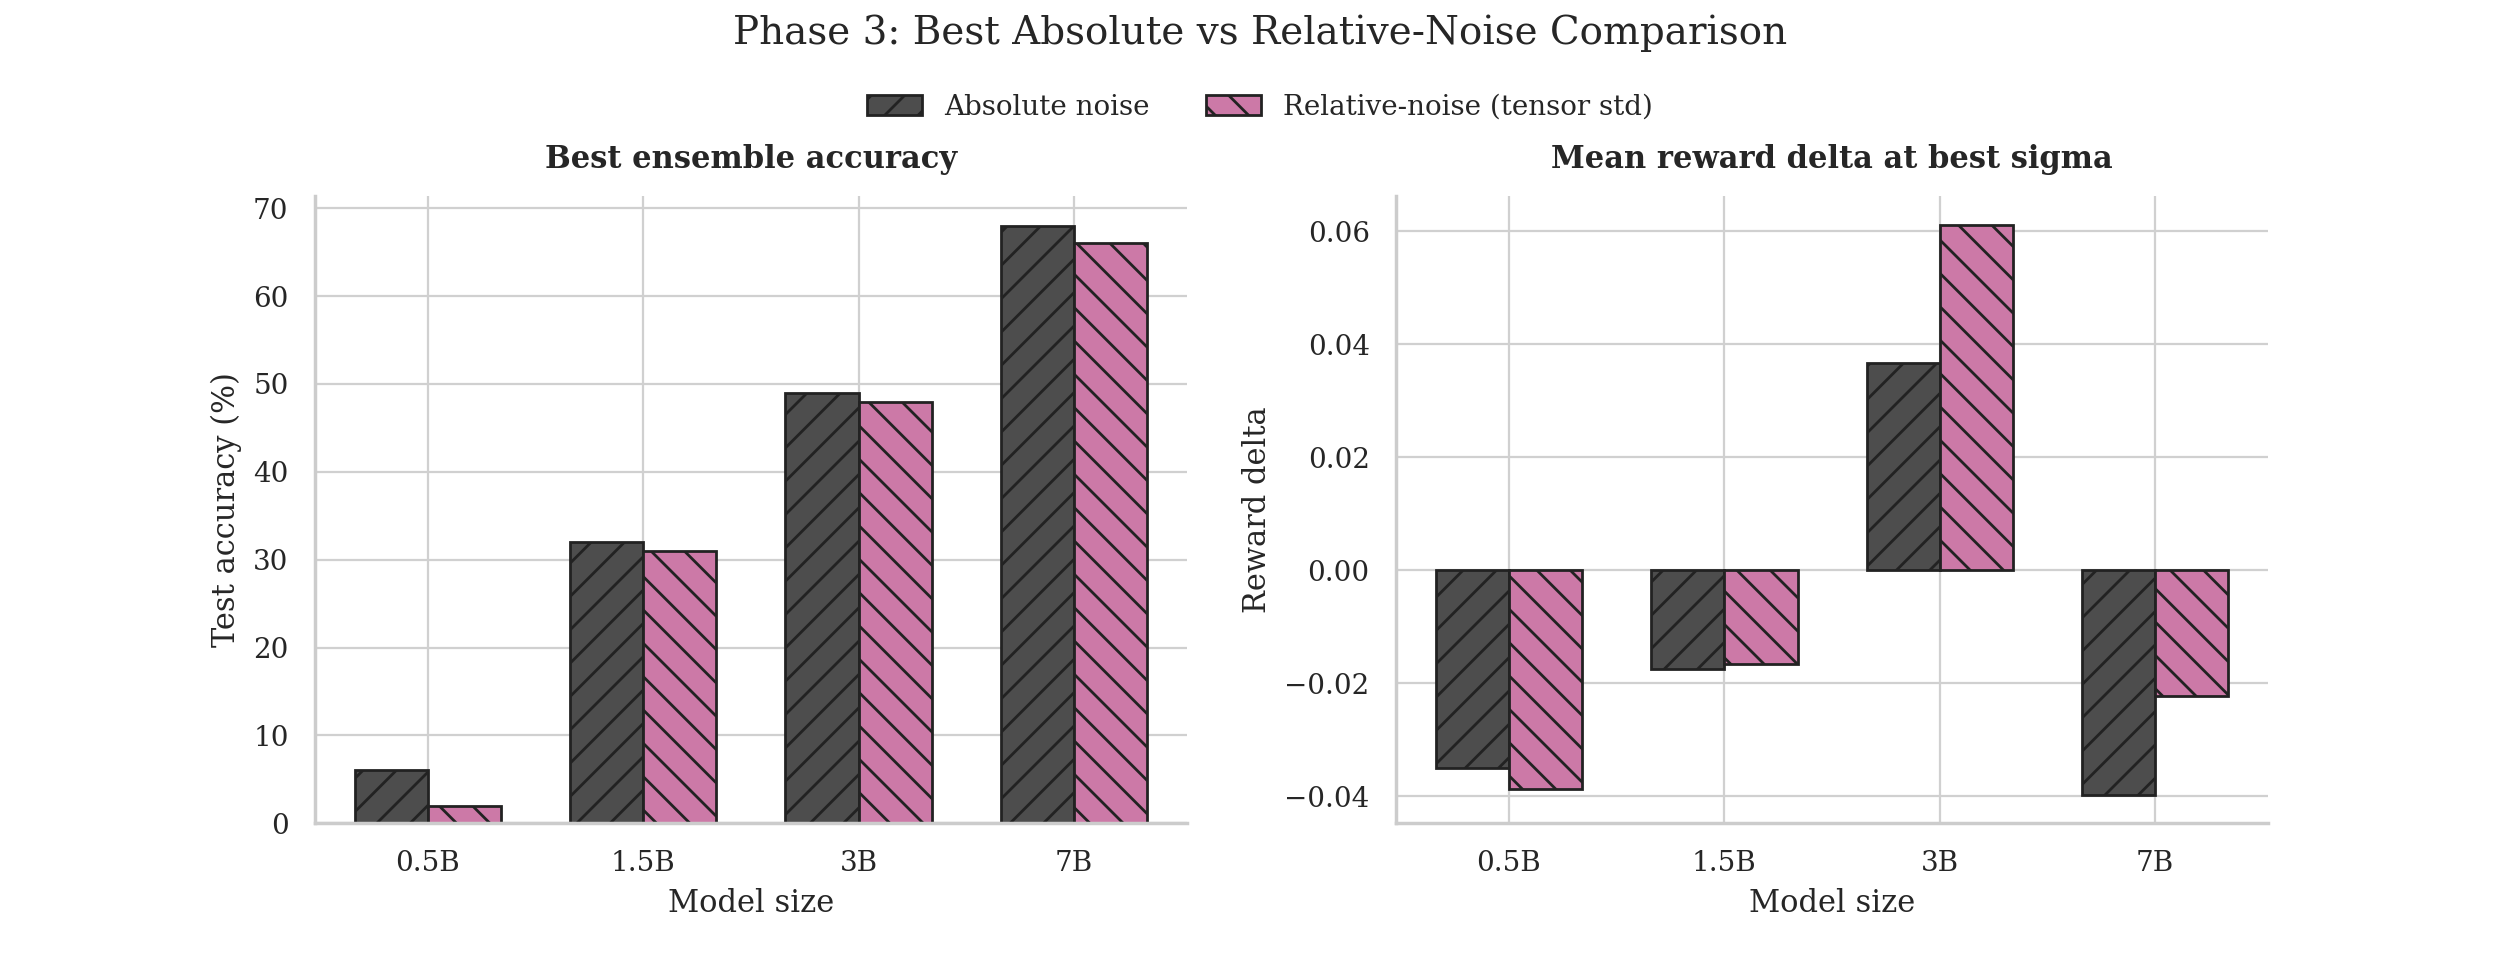
\includegraphics[width=0.85\textwidth]{figures/phase3_comparison.png}
\caption{Best ensemble accuracy (left) and mean reward delta (right) under absolute vs.\ relative-norm perturbations, each at its respective optimal $\sigma$. The two perturbation families produce very similar results at each scale.}\label{fig:phase3}
\end{figure}

Figure~\ref{fig:phase3} compares the best results from each perturbation family. The two schemes produce nearly identical peak ensemble accuracies: 32\% vs.\ 31\% at 1.5B, 49\% vs.\ 48\% at 3B, 68\% vs.\ 66\% at 7B. The choice of perturbation parameterization did not materially change the Countdown results in our tested setup (one task, one model family, narrow sigma grid).

\paragraph{A note on norm layers.} The relative-norm initial grid ($\sigma\in\{0.05, 0.1, 0.2, 0.5\}$) turned out to be far too destructive---near-zero rewards even at $\sigma=0.05$---because it perturbed norm layers by $\sigma_{\text{eff}}\approx 0.05\times 0.3 = 0.015$, well into the destructive range. This is itself informative: the norm layers appear to be sensitive to perturbation, and the paper's absolute-noise scheme may work partly \emph{because} it leaves norms nearly untouched.


\section{Summary}

\begin{table}[ht]
\centering
\small
\caption{Status of the paper's core claims after our investigation.}\label{tab:summary}
\begin{tabular}{p{4.5cm} p{1.5cm} p{7.5cm}}
\toprule
\textbf{Claim} & \textbf{Status} & \textbf{Notes} \\
\midrule
Thickets exist (task-improving solutions are nearby) & Supported & Survives RNG fix. $K=1$ accuracy scales with model size under the corrected sampler with appropriate $\sigma$. Hit-rate scaling is less clean at stricter margins. \\
\addlinespace
Density scales monotonically at fixed $\sigma$ (Eq.~\ref{eq:density}) & Confounded & The paper's $\sigma=0.005$ appears destructive under the corrected sampler (inferred from bracketing grid points). The underlying phenomenon is plausible but the paper's specific measurement (fixed $\sigma$) does not cleanly establish it. \\
\addlinespace
RandOpt is competitive & Plausible & Works under the corrected sampler with $\sigma\approx 0.001$, but we did not compare against PPO/GRPO/ES and used smaller $N$, $K$ than the paper. \\
\addlinespace
Diversity / Spectral Discordance & Untested & Requires multi-task evaluation; out of scope. \\
\bottomrule
\end{tabular}
\end{table}

The released implementation does not match the paper's stated perturbation distribution (Section~\ref{sec:rng}). Despite this, useful nearby task-improving solutions still exist after fixing the sampler: $K=1$ test accuracy on Countdown scales monotonically with model size when each model is evaluated at its own optimal $\sigma$ (Figure~\ref{fig:k1_vs_sigma}). Correcting the RNG changes the optimal $\sigma$ but does not destroy the phenomenon.

However, the paper's specific density scaling law---measured by hit-rate at a single fixed $\sigma=0.005$---is not cleanly established by our reproduction. Our sigma sweep suggests that $\sigma=0.005$ is at or beyond the destructive regime for all models under the corrected sampler (inferred from bracketing grid points at $\sigma=0.003$ and $\sigma=0.01$), and that the productive regime is roughly an order of magnitude smaller ($\sigma\approx 0.001$). Furthermore, while $K=1$ accuracy scales monotonically, the hit-rate measure $\delta(m)$ does not show clean monotonic scaling at stricter accuracy margins (Figure~\ref{fig:hitrate_vs_sigma}). The density scaling claim requires each model to be evaluated at an appropriate perturbation scale; the paper's fixed-$\sigma$ design confounds genuine geometric structure with noise robustness. A simple theoretical argument based on the $\mu$P scaling of perturbation impact (Appendix~\ref{app:norms}) predicts that optimal $\sigma$ should decrease as $1/\sqrt{\text{width}}$, though our sigma grid is too coarse to test this quantitatively.

\paragraph{Limitations.} Our experiments use a single task (Countdown), a single model family (Qwen-2.5), and modest sample sizes ($N=100$--$200$, vs.\ the paper's $N=1000$--$5000$). Our $K=1$ results understate what larger ensembles can achieve---the paper's $K=50$ results are substantially stronger, particularly at 0.5B where we observe near-zero $K=1$ accuracy but the paper reports 8.4\% with $K=50$. We did not test the diversity claim, and we did not compare against gradient-based baselines. Our results are consistent with the paper's qualitative conclusions but we cannot rule out that the picture differs on other tasks or model families.


\bibliographystyle{plain}
\bibliography{references}


\appendix

\section{What Norm Should Perturbations Be Measured In?}\label{app:norms}

The paper defines solution density (Eq.~\ref{eq:density}) in terms of isotropic Gaussian perturbations in raw parameter space. This is implicitly a Frobenius-norm neighborhood: adding $\boldsymbol{\epsilon}\sim\mathcal{N}(\mathbf{0},\sigma^2\mathbf{I})$ to a weight matrix $W\in\mathbb{R}^{n\times m}$ produces a perturbation whose Frobenius norm is $\|\sigma E\|_F \approx \sigma\sqrt{nm}$, scaling with the total number of entries. But this is not obviously the right measure of perturbation size for a linear operator.

\paragraph{A single-matrix toy model.} Consider a single linear layer $y = Wx$ with $W\in\mathbb{R}^{n\times n}$ and input $x\in\mathbb{R}^n$ with $\|x\|\approx\sqrt{n}$ (typical after layer norm). Add perturbation $\sigma E$ with $E_{ij}\sim\mathcal{N}(0,1)$. Each output entry is perturbed by
\[
  \Delta y_j \;=\; \sigma\sum_i E_{ji}\, x_i, \qquad \mathrm{Var}(\Delta y_j) = \sigma^2\|x\|^2 \approx \sigma^2 n.
\]
So $\mathrm{std}(\Delta y_j)\approx \sigma\sqrt{n}$: the functional impact of per-parameter noise grows with $\sqrt{\text{width}}$. To keep the output perturbation constant across different widths, one needs $\sigma\propto 1/\sqrt{n}$.

This is the same scaling that appears in the spectral norm of the perturbation. By the Marchenko--Pastur law, the largest singular value of $\sigma E$ is $\|\sigma E\|_*\approx 2\sigma\sqrt{n}$. The spectral norm measures how much the matrix's action on vectors changes---i.e., the worst-case amplification of any input direction---and it grows as $\sigma\sqrt{n}$ even though each entry was only perturbed by $\sigma$.

\paragraph{Connection to $\mu$P.} This scaling is well-known in the maximal update parameterization ($\mu$P) literature~\cite{yang2023spectral}, where the prescription for weight updates is: the spectral norm of the update $\|\Delta W\|_*$ should be $\Theta(1)$ as width grows, which requires per-entry learning rates to scale as $1/\sqrt{\text{width}}$. The same logic applies to random perturbations: to keep the functional impact of a perturbation constant across model scales, $\sigma$ should scale as $1/\sqrt{\text{width}}$.

\paragraph{For a full transformer.} With $L$ layers and residual connections, output perturbations from independent per-layer noise accumulate roughly additively, giving total functional perturbation $\propto\sigma\cdot\sqrt{\text{width}}\cdot L$. This suggests
\[
  \sigma_{\text{optimal}} \;\propto\; \frac{1}{\sqrt{\text{width}}\cdot L}
\]
to maintain constant functional impact. Plugging in Qwen-2.5 architectures:

\begin{center}
\small
\begin{tabular}{lccc}
\toprule
Model & Width & Layers & $1/(\sqrt{\text{width}}\cdot L)$ \\
\midrule
1.5B & 1536 & 28 & $9.1\times 10^{-4}$ \\
3B   & 2048 & 36 & $6.1\times 10^{-4}$ \\
7B   & 3584 & 28 & $6.0\times 10^{-4}$ \\
\bottomrule
\end{tabular}
\end{center}

This predicts that 3B and 7B should use roughly 2/3 the $\sigma$ of 1.5B, and that 3B and 7B should be similar (7B is wider but shallower). Our sigma sweep found $\sigma\approx 0.001$ optimal for all three, but the grid was too coarse to resolve a 1.5$\times$ difference.

\paragraph{Caveats.} We do not claim the spectral norm is definitively the right metric---other choices (Fisher Information, KL divergence, per-tensor relative scaling) are also defensible and may give different prescriptions. The point is that there are simple theoretical reasons to expect $\sigma$ to depend on model architecture, and that the paper's fixed-$\sigma$ choice does not account for this.

\end{document}
